\section{Theorie}
\label{sec:theorie}

Als Interferenz wird die Eigenschaft von Licht bezeichnet, bei Überlagerung die Amplitude zu ändern.
Dabei werden die Amplituden zweier oder mehrerer Wellen addiert.\\
Die Interferometrie nutzt diese Eigenschaft, um das Licht selbst zu untersuchen oder um materialspezifische Eigenschaften von Materie zu analysieren.

\subsection{Kohärenz}
Um Interferenz effektiv auszunutzen, ist es nötig die Kohärenz des Lichts zu betrachten.
Licht ist dann kohärent, wenn sich die Auslenkungen der Wellen, bis auf einen konstanten Phasenunterschied, zeitlich an verschiedenen Orten gleich ändern.
Zusätzlich muss die Wellenlänge aller individuellen Wellenpakete gleich sein.\\
\newline
Bei zeitlicher Kohärenz bleibt die Phasendifferenz in Ausbreitungsrichtung konstant, was durch die Kohärenzzeit $\tau_c$ bestimmt ist.
Diese gibt an, ab welchem Zeitpunkt die Phasendifferenz nicht mehr konstant bleibt und die Kohärenz sinkt.
Für die Kohärenzzeit $\tau_c$ gilt:
\begin{equation}
    \tau_c = \frac{1}{\Delta \nu} \qquad \text{mit} \qquad \Delta \nu \equiv \text{Bandbreite des Lichts}
\end{equation}
\newline
Bei räumlicher Kohärenz hat die Lichtwelle zum gleichen Zeitpunkt an verschiedenen Orten die selbe Amplitude.\\
In \autoref{fig:coherencea} und \ref{fig:coherenceb} wird graphisch der Unterschied zwischen zeitlicher und räumlicher Kohärenz dargestellt.

\begin{figure}[H]
    \begin{subfigure}{.5\textwidth}
        \centering
        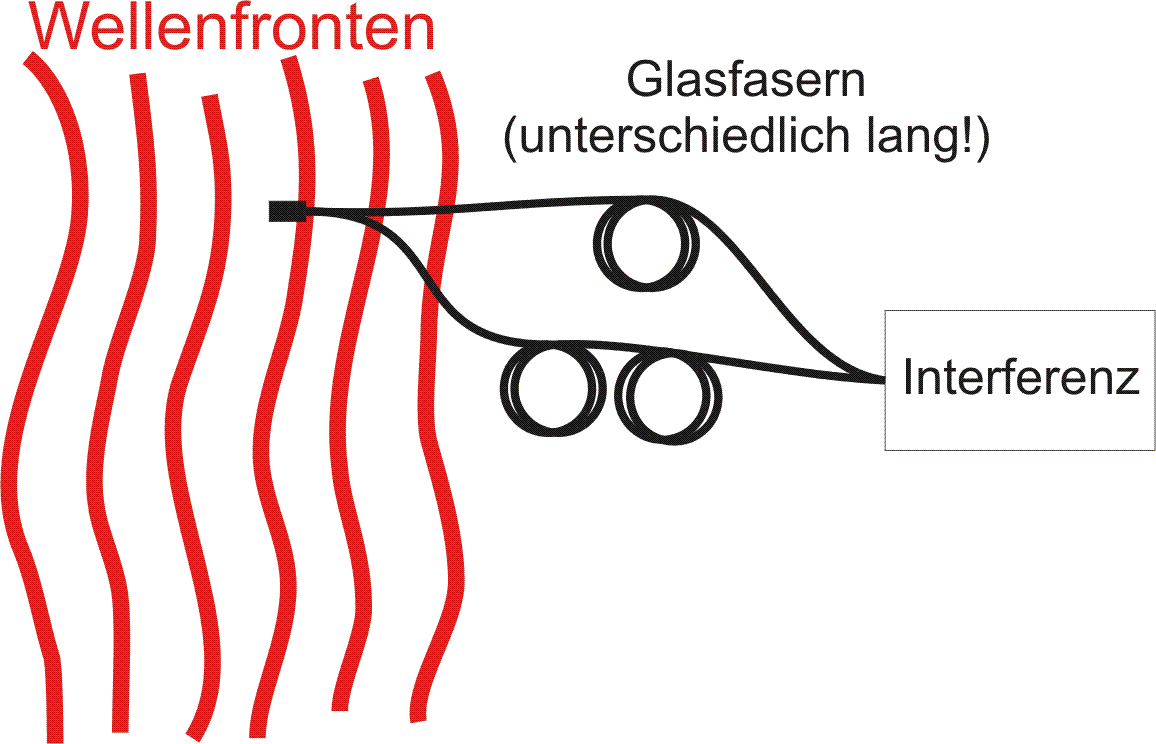
\includegraphics[scale=0.15]{images/zeitco.png}
        \caption{Darstellung von zeitlicher Kohärenz.\cite{koharenz}}
        \label{fig:coherencea}
    \end{subfigure}
    \begin{subfigure}{.5\textwidth}
        \centering
        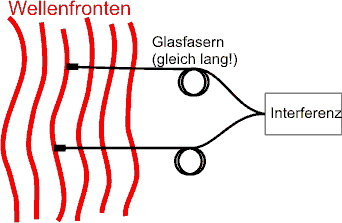
\includegraphics[scale=0.5]{images/raumco.png}
        \caption{Darstellung von räumlicher Kohärenz.\cite{koharenz}}
        \label{fig:coherenceb}
    \end{subfigure}
\end{figure}

Zusätzlich zur Kohärenzzeit lässt sich die Kohärenz auch mit einem Kontrast $V$ des Interferenzmusters beschreiben.
Bei maximalem Kontrast ist das Licht vollständig kohärent, bei Minimalem vollständig inkohärent.
Der Kontrast berechnet sich aus den Intensitäten des Lichts und dem Kohärenzgrad
\begin{equation}
    \Gamma = \langle E_1 E_2^\dagger \rangle \quad \text{,} \quad \gamma = \frac{\Gamma}{\sqrt{I_1 I_2}}
    \label{eq:grad}
\end{equation}
, und es gilt:
\begin{equation}
    V = \frac{2\sqrt{I_1I_2}}{I_1 + I_2}|\gamma|
    \label{eq:kontrast_formel}
\end{equation}
Wird vollständig kohärentes Licht angenommen, gilt für den Kontrast auch \autoref{eq:kontrast}.
\begin{equation}
    V = \frac{I_{max} - I_{min}}{I_{max} + I_{min}}
    \label{eq:kontrast}
\end{equation}
Vollständig kohärentes Licht ist nur theoretisch, da Lichtquellen nicht eindeutig monochromatisch leuchten.
Da es nur teilmonochromatisches Licht gibt, gibt es dahingehend auch nur Teilkohärenz.

\subsection{Fresnel-Arago-Gesetze}
Die Fresnel-Arago-Gesetze befassen sich mit der Polarisation des Lichts bei Interferenz.\\
Licht ist in der Regel unpolarisiert und wird deswegen in einen senkrechten und horizontalen Polarisationsanteil aufgespalten.
Auch für polarisiertes Licht mit integrierter Phasenverschiebung, wie zum Beispiel zirkulär polarisiertem Licht, ist das möglich, wobei die Phasenverschiebung erhalten bleibt.\\
Die vier Gesetze von Augustin Jean Fresnel und François Arago befassen sich mit zwei Lichtstrahlen und deren Polarisation zueinander, um deren Interferenz zu bestimmen.
Sie lauten zusammengefasst:
\begin{itemize}
    \item Zwei linear polarisierte Lichtstrahlen mit zueinander parallelen Polarisationsebenen, interferieren wie nicht polarisiertes Licht.
    \item Zwei linear polarisierte Lichtstrahlen mit zueinander senkrechten Polarisationsebenen, interferieren nicht.
    \item Zwei zueinander senkrecht linear polarisierte Lichtstrahlen, interferieren nur dann, wenn sie aus einem Strahl kamen und erneut zu einem Strahl mit selber Polarisationsebene zusammengeführt werden.
    \item Zwei zueinander senkrecht linear polarisierte Lichtstrahlen, interferieren bei Zusammenführung nicht, wenn sie aus nicht polarisiertem Licht entstanden sind.
\end{itemize}

\subsection{Interferenzbild}
